%\stepcounter{contsubsec} 
\section{ Planteamiento del problema}

Se refiere al interrogante que lleva al investigador a buscar respuestas concretas. Es la definición del problema que aborda con la investigación.

La presente plantilla de \LaTeX, como cualquier documento de formato \textit{.tex} necesita un editor de \LaTeX\ ya sea instalado en su dispositivo o un editor online. Como todos los archivos se necesitan entre sí, todos los que aquí se encuentran debe ser subidos o leídos por su editor, además de la carpeta con las imágenes ya que algunos comandos usan la ruta de ella (del tipo: imagenes/imagen.jpg)\footnote{Si tienes dudas, solicita asesoría en biblioteca, CRAI o centro de documentación respectivo}. Además, recomendamos tener especial cuidado con los archivos \textit{macros.tex} y \textit{apaudea.bst}, estos dos soportan toda la estructura general de la plantilla y los parámetros de las normas APA; cualquier modificación, por mínima que sea de ellos, puede generar severos problemas en la compilación.

Está plantilla de \LaTeX \ fue creada con divisiones en secciones, donde el primer nivel es la división \textit{$\setminus$section\{\}} , la de segundo nivel \textit{$\setminus$subsection\{\}}, \textit{$\setminus$subsubsection\{\}}, \textit{$\setminus$paragraph\{\}} y \textit{$\setminus$subparagraph\{\}} los tres siguientes niveles; asegúrese usar esta división para que se puedan cargar cada partición en la tabla de contenido de forma automática; si escribe los diferentes títulos sin estos comandos, deberá cosntruir la tabla de contenido

Recuerde que el \LaTeX\  también tiene la herramienta de divisiones con *, las cuales aparecen en el documento con su respectivo título y no aparecen en la tabla de contenido

\subsection{Antecedentes}

Los antecedentes son las investigaciones que se han realizado previamente y que guardan una relación histórica con el tema de investigación actual. 

\newpage
%-------------------------------


\section{Justificación}

Responde a los interrogantes del por qué se desea conocer el tema y por qué se seleccionó, así como cuál es el aporte que tendrá el texto a la ciencia. 

No abuse del uso de \textit{cursivas} o \textbf{negritas} dentro del texto, úselas muy moderadamente, por lo general saturan y dificultan la lectura del documento. Utilice cursivas en casos muy particulares como géneros y especies (\textit{Tyrannus melancholicus}), términos químicos (\textit{kr}), letras griegas ($\beta$) y algunos títulos y subtítulos. El entorno matemático de \LaTeX \ muestra las variables y símbolos en letra cursiva, asegurese de hacer lo mismo al referenciarla en el documento, Utilice \textbf{negritas} en algunos títulos de capítulos y subcapítulos, algunos datos de tablas o enfatizar aspectos muy particulares. El uso de \underline{texto subrayado} no se recomienda en normas APA.

Utilice moderadamente el uso de abreviaturas, se prefiere que el texto sea más largo y claro que corto y confuso para el lector. Por ejemplo, APA puede significar American Psychological Association o American Psychiatric Association. Sin embargo, las abreviaturas pueden ser útiles en casos como la repetición continua en un mismo párrafo.

Prefiera las comillas “inglesas” y ‘sencillas’ por sobre las «latinas» o «españolas».

\begin{description}
    \item[Características:] texto descriptivo.
    \item[Propiedades:] texto descriptivo.
    \item[Estructura:] texto descriptivo.
\end{description}

\newpage
%--------------------------
\section{Objetivos}

\subsection{Objetivo general}

El objetivo general y los objetivos específicos describen lo que se pretende con la investigación, cuál es el alcance y cuál es el problema que se desea resolver. Deben iniciarse con verbos que describan claramente lo que se lleva a cabo.

\subsection{Objetivos especificos}

Se describen algunos ejemplos de verbos comunes que se utilizan en el planteamiento de objetivos, los cuales cambiarán dependiendo de su investigación.

\begin{itemize}
    \item Describir.
    \item Analizar.
    \item Demostrar.
    \item Probar.
    \item Comparar.
    \item Definir.
    \item Establecer.
    \item Interpretar.
\end{itemize}

\newpage
%--------------------------
\section{Problema de investigación}

El problema de investigación es el enunciado de lo que puede ser demostrado o encontrado, y de lo cual se requieren pruebas y evidencias.

\newpage
%--------------------------
\section{Hipótesis}

La hipótesis es la creencia, la suposición o la conjetura de un fenómeno posible, es decir, independiente de si es verdadero o no. En la hipótesis se reúnen datos, se comparan y se escogen las explicaciones más probables. Dicho de otra forma, la hipótesis es la explicación probable de la relación entre dos o más variables.

    \subsection{Hipótesis de trabajo}

    Texto descriptivo.

    \subsection{Hipótesis estadística}

    Texto descriptivo.
    
    \subsubsection{Hipótesis nula}

    Texto descriptivo.

        \paragraph{Hipótesis alterna. }
        
        Texto descriptivo inicia en la misma línea y continúa como párrafo normal APA.
        
        \subparagraph{Variables.}
        
        Texto descriptivo inicia en la misma línea y continúa como párrafo normal APA.

\newpage
%--------------------------
\section{Marco teórico}

En esta sección se citan los autores que han tenido influencia directa en tu investigación. Recuerda, debes escoger solo un método para realizar las citas y referencias, es decir, debes seleccionar entre gestores especializados como Mendeley, Zotero, EndNote, etc., Microsoft Word, o “Manuales”; no se deben mezclar entre sí. Nuestra recomendación principal es Mendeley. Evita referenciar sitios como blogs, Wikipedia, Rincón del Vago, Monografías.com y demás portales web que no se consideran fuentes primarias. No limites tu búsqueda a una sola herramienta (por ejemplo, solo www.google.com). Realiza búsquedas en diferentes plataformas académicas, tales como:

\begin{itemize}
    \item \textbf{Catálogo Sistema de Bibliotecas UdeA:} material impreso que reposa en Bibliotecas UdeA, tales como libros, revistas, tesis, diccionarios, informes, etc.
    \item\textbf{Bases de datos suscritas de la Biblioteca:} plataformas digitales con millones de documentos en texto completo.
    \item\textbf{Bases de datos de libre acceso:} Google Scholar, Microsoft Academic, Google Books, Redalyc, Scielo, Dialnet, DOAJ, PubMed, Base Search, entre muchas más.
    \item\textbf{Documentos con acceso restringido:} si requieres el texto completo de artículos o libros con acceso restringido, que por lo general se encuentran en bases de datos no suscritas por la Universidad de Antioquia, solicítalos en tu Biblioteca enviando título exacto, el DOI o la url del documento. Tenemos convenios nacionales e internacionales que nos permiten acceder a esta información.
\end{itemize}

Ejemplo de cita parafraseada, es decir, frase no textual adaptada con las palabras de quien escribe; esta forma de citación es la más adecuada en textos académicos, demuestran lectura, análisis y redacción propia (Arango, 2000). Ejemplo de “Cita textual menor a 40 palabras, al interior del párrafo. No utilice recurrentemente esta forma de citación, pues demuestra poco análisis y redacción propios” (Ramírez H. \& Guzmán, s.f., p. 9). Otros ejemplos aceptados en estilo APA 7:

Un autor en paráfrasis (Arango, 2000), dos autores en paráfrasis (Ramírez H. \& Guzmán, s.f.), tres o más autores en paráfrasis (Baker et al., 2002), cita en paráfrasis sin fecha (Ramírez H. \& Guzmán, s.f.), cita en paráfrasis con dos o más fuentes en un solo paréntesis, en orden alfabético, separados por punto y coma (Fundación del Español Urgente [Fundéu]; Hooper, 2010; Institute of Electrical and Electronics Engineers [IEEE], 2006).

Un autor en “cita textual menor a 40 palabras” (Arango, 2000, p. 466), dos autores en “cita textual menor a 40 palabras” (Ramírez H. \& Guzmán, 2015, p. 2), tres o más autores en “cita textual menor a 40 palabras” (Baker et al., 2002, p. 1281), autor corporativo en “cita textual de sitio web con número de párrafo” (El Espectador, 2012, párr. 9), cita “textual menor o mayor a 40 palabras omitiendo fragmentos intermedios (…) entre paréntesis y tres puntos” (Ruiz Rojas, 2014, p. 45), cita “textual menor a 40 palabras con páginas continuas” (Rioja, 2008, pp. 15-16), cita “textual menor a 40 palabras con páginas discontinuas” (González Pérez et al., 2006, pp. 15, 17).

Autor corporativo sin siglas reconocibles en paráfrasis (Biblioteca Universidad de San Buenaventura, 2016), autor corporativo en paráfrasis, nombre completo, con sigla reconocida entre corchetes, primera cita (International Business Machine [IBM], 2013), las citas subsiguientes solo con la sigla reconocida entre paréntesis (IBM, 2013).

Cita de cita en paráfrasis (Quintero \& González, 1997, citados por Rioja, 2008), cita de cita “textual menor a 40 palabras” (Quintero \& González, 1997, citados Rioja, 2008, p. 36). Cita textual mayor a 40 palabras sin comillas:

    \begin{quotation}
    Por su parte la necesidad de persuadir conduce a pensar el material probatorio dependiendo del ánimo de quien escucha. En síntesis, el componente lógico se fundamenta en la selección de argumentos verosímiles, lo cual conduce directamente al componente dialéctico de la argumentación en tanto la parte psicológica remite a un aspecto discursivo. (Ruiz Rojas, 2014, p. 107) 
    \end{quotation}

Las comunicaciones personales corresponden a cartas, memorandos, correos electrónicos, conversaciones telefónicas, entrevistas, presentaciones inéditas de clases, entre otras fuentes inéditas, que no proporcionan datos recuperables; se citan, pero no se incluyen en el listado de referencias (J. C. Ramírez, comunicación personal, 4 de julio, 2020).

\newpage
%--------------------------
\section{Métodos para elaborar citas y referencias }

Recuerda, debes escoger solo un método para realizar las citas y las referencias, es decir, debes seleccionar entre un gestor especializado como Mendeley, Zotero o EndNote (confiabilidad alta), el gestor nativo Microsoft Word (confiabilidad media) o “manuales” (confiabilidad baja); no se deben mezclar entre sí, nuestra recomendación principal es Mendeley, pues te permite almacenar, subrayar e insertar notas en PDF´s, guardar fichas bibliográficas, elaborar citas y bibliografías en APA, Vancouver, IEEE y más de 1.000 estilos diferentes, exportar registros, compartir documentos, etc. Para mayor información de Mendeley.com y \LaTeX visitar:

\url{http://tiny.cc/zzrnuz}

La presente plantilla incluye los archivos requeridos para la construcción apropiada de las referencias bibliograficas bajo los parametros de las normas APA, todo se limita a modificar los campos del archivo \textit{refe.bib} segun las necesidades de su escrito. Aqui algunos ejemplos de los diferentes tipos de documentos referanciables.

Refencia a un libro \citep{lib:libro},  a un acta \citep{act:acta}, a un artículo \citep{art:articulo}, a una conferencia \citep{con:conferencia}, a un capítulo o páginas específicas con título propio de un libro\citep{ent:entre_libro}, a una seccion de libro sin título \citep{sec:seccion_libro}, a un documento sin editorial \citep{fll:folleto}, a las memorias de una conferencia \citep{ina:articulo_en_acta}, a un informe técnico \citep{inf:informe_tecnico}, a un manual \citep{man:manual}, a una tesis doctoral \citep{phd:phd_tesis}, a una tesis de maestría \citep{tes:tesis}, a una web o información de internet \citep{web:web}, y para otros tipos de referencias diferentes a las anteriores \citep{opc:opcional}. El apellido principal será la última palabra en el campo \textit{author}, tanto para la citación en el texto como para la lista de referencias y su organización alfabética; Si como autor no figura una persona sino una organización, al llenar el campo \textit{author} del archivo \textit{.bib}, use $\{\}$ dobles (ver referencia \citep{lib:apa}).

A continuación se muestra una de las referencias del archivo \textit{refe.bib}, donde \linebreak {\textit{ent:entre\_libro}} es el identificador de la misma y para referenciarla se debe escrbir el comando $\backslash citep\{ent:entre\_libro\}$ 

\newpage
\begin{verbatim}
@inbook{ent:entre_libro,
     author         = {Angela Zapata},
     title          = {Titulo de libro},
     chapter        = {},
     pages          = {10-20},
     publisher      = {Editor},
     volume         = {},
     series	        = {},
     type           = {},
     address        = {},
     edition        = {},
     year           = {20XX},
     month          = {},
     note           = {},
     language       = {},
     }
\end{verbatim}

con respecto a citas y referencias de material legal, diríjase al anexo 2, algunos ejemplos serían \citepLegal{leg:constitucion} y  \citepLegal{leg:minambiente} \citepLegal{leg:ley133} \citepLegal{leg:decreto1504} \citepLegal{leg:ley1733} \citepLegal{leg:sentenciaSU805} \citepLegal{leg:SentenciaT361} \citepLegal{leg:SentenciaT264} \citepLegal{leg:resolucion4331} \citepLegal{leg:circular048} \citepLegal{leg:iluminacion} \citepLegal{leg:espanalaborales}

Recuerde que \LaTeX , en la sección de referencias, solo muestra las que se han citado en su escrito; agregar la información en el archivo \textit{refe.bib} no implica que la referencia se muestre en su documento




\newpage
%--------------------------
\section{Metodología}

En la metodología se establecen los enfoques de investigación, esto es, cuantitativo, cualitativo o mixto.

\newpage
%--------------------------
\section{Resultados}

En los resultados se comunican los hallazgos y descubrimientos del estudio. Se incluyen tablas, figuras, diagramas y demás material demostrativo.


\begin{equation}
    \oint_C \vec{B}\cdot d \vec{l}=\mu_0\int_S \vec{J}\cdot d \vec{s}+\mu_0\epsilon_0\dfrac{d }{d t}\int_S \vec{E}\cdot d \vec{s}
\end{equation}

y a su vez

\begin{gather}
    \vec{\nabla}\cdot \vec{E}= \dfrac{\rho}{\epsilon_0}\\
    \vec{\nabla}\cdot \vec{B}= 0\\
    \vec{\nabla}\times\vec{E}=-\dfrac{\partial\vec{B}}{\partial t}\\
    c^2\vec{\nabla}\times\vec{B} =\dfrac{\vec{J}}{\epsilon_0}+\dfrac{\partial
\vec{E}}{\partial t}\\
    \vec{\nabla}\times \vec{B}=\mu_0\vec{J}+\mu_0 \epsilon_0 \dfrac{\partial \vec{E}}{\partial t}
\end{gather}

 Al narrar descriptivamente una figura, tabla, etc., en un párrafo, puedes insertar una referencia cruzada, es decir, un hipervínculo al elemento mencionado dentro o fuera de paréntesis, ejemplos: estos resultados se muestran en la Tabla \ref{table:prob_milenio}.  Igualmente, los datos son validados con otros instrumentos (Tabla \ref{table:num_mersenne}, Tabla \ref{table:medalla_fields}). Lineamientos que se establecen en la nueva versión de las Normas APA séptima edición (Figura \ref{figportada_apa}). La producción intelectual institucional se publica en el Repositorio (Figura \ref{fig:escudo_udea}). Si la figura es de tu completa autoría, \textbf{NO} es necesario colocar la leyenda “Elaboración propia” (Figura \ref{fig:hiperbolica}).

\begin{figure}[!ht]
\caption{Función hiperbólica}
    \begin{center}
    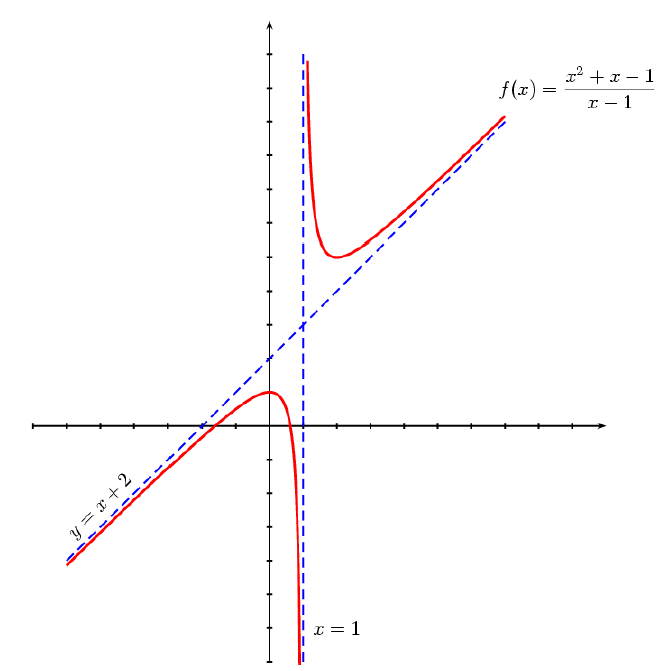
\includegraphics[scale=0.5]{imagenes/grafica.png}\\
    \label{fig:hiperbolica}
    \end{center}
    \textit{}
\end{figure}

\begin{table}%[!ht]
\caption{Problemas del milenio: la resolucion de uno de estos problemas se premian con un monto de us\$ 1 millon}
\begin{center}
\begin{tabular}{  l c }
    \hline
    1 & El problema de $P$ frente a $NP$  \\ \hline
    2 &  La conjetura de Hodge \\ \hline
    3 &  La conjetura de Poincaré \\ \hline
    4 &  La hipótesis de Riemann \\ \hline
    5 &  Yang-Mills y el salto de masa ("mass gap")\\ \hline
    6 &  Las ecuaciones de Navier-Stokes\\ \hline
    7 &  Conjetura de Birch y Swinnerton-Dyer\\
        \hline
\end{tabular}
\end{center}
\label{table:prob_milenio}
\end{table}

%\clearpage

\begin{table}%[!ht]

\caption{Medalla Fields: matemáticos galardonados con este premio desde 2002; la medalla Fields se comenzó a entregar desde 1936}
\begin{center}
\begin{tabular}{cp{4cm}p{2.5cm}p{6cm}}
    \hline
    año & Ganador(es) & pais & universidad/instituto\\
    \hline 
    2002 & Vladimir Voevodsky  & Rusia &Instituto de Estudios Avanzados de Princeton \\
         & Laurent Lafforgue & Francia &Institut des hautes études scientifiques \\ 
         \hline
        2006 & Andrei Okounkov & Rusia & Universidad de Princeton\\
         & Grigori Perelmán (rechazó el premio) & Rusia & Instituto de Matemáticas Steklov\\
         & Terence Tao & Australia & Universidad de California, Los Ángeles \\
         & Wendelin Werner  & Francia & Université de Paris-Sud\\
         \hline
        2010 & Elon Lindenstrauss & Israel & Universidad Hebrea de Jerusalén\\
         & Ngô Bảo Châu ,  & Vietnam y Francia &Paris-Sud 11 University y Institute for Advanced Study \\
         & Stanislav Smirnov  & Rusia & Universidad de Ginebra\\
         & Cédric Villani & Francia & Institut Henri Poincaré\\
         \hline
         2014 & Artur Ávila  & Francia &Instituto Nacional de Matemática Pura y Aplicada \\
         & Manjul Bhargava  &  Canadá y Estados Unidos &Universidad de Princeton \\
         & Martin Hairer & Austria & Imperial College London\\
         & Maryam Mirzajani & Irán &Universidad Stanford \\
         \hline\\
         2018	 & Caucher Birkar & Irán y Reino Unido & Universidad de Cambridge \\
         & Alessio Figalli & Italia & Escuela Politécnica Federal de Zúrich \\
         & Peter Scholze & Alemania & Universidad de Bonn\\
         & Akshay Venkatesh  & Australia & Universidad Stanford\\
        \hline
\end{tabular}
\end{center}
\label{table:medalla_fields}
\end{table}

\clearpage

\begin{table}%[!ht]
\caption{Algunos números primos de Mersenne}
\begin{center}
\begin{tabular}{ c|c}
    \hline
    Exponente $n$ & Primo de Mersenne \\ \hline
    2 &  $2^{2}-1=3 $ \\ \hline
    3 &  $2^{3}-1=7 $ \\ \hline
    5 &  $2^{5}-1=31 $ \\ \hline
    7 &  $2^{7}-1=127 $ \\ \hline
    13 &  $2^{13}-1=8191 $ \\ \hline
    17 &  $2^{17}-1=131071 $ \\
        \hline
\end{tabular}
\end{center}
\label{table:num_mersenne}
\end{table}


\begin{figure}[!ht]
\caption{Portada Normas APA séptima edición 2020 en inglés}
    \begin{center}
    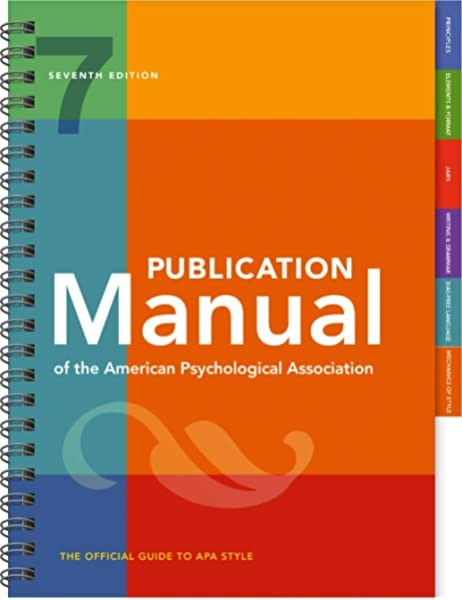
\includegraphics[scale=0.4]{imagenes/portadaAPA2020.jpg}\\
    \label{figportada_apa}
    \end{center}
    \textit{Nota.} Fuente https://bit.ly/2IyrZao \citep{lib:apa}.
\end{figure}

\clearpage

\begin{figure}[!ht]
    \caption{Logo Universidad de Antioquia}
    \begin{center}
    
\includegraphics{imagenes/escudo_udea_solo.png}\\
    \label{fig:escudo_udea}    
    \end{center}
    \textit{Nota.} Fuente http:/www.udea.edu.co
\end{figure}

\clearpage

%--------------------------
\section{Discusión}

La discusión es la interpretación crítica y el análisis de los resultados, que surgen de las preguntas de investigación.


\newpage
%--------------------------
\section{Conclusiones}

Son las interpretaciones finales que recopilan los datos de la investigación, describe lo que se obtuvo, qué se logró y cuáles son los resultados. Guardan relación directa con lo que se mencionó en el planteamiento del problema. Pueden confirmar las hipótesis. 


\newpage
%--------------------------
\section{Recomendaciones}

Las recomendaciones son las futuras y posibles líneas de investigación que llevarán a resolver problemas relacionados con la presente investigación.


